\documentclass[../main.tex]{subfiles}
\begin{document}
\section{Methods}
\labsec{methods}

\subsection{Architecture of CNN network}
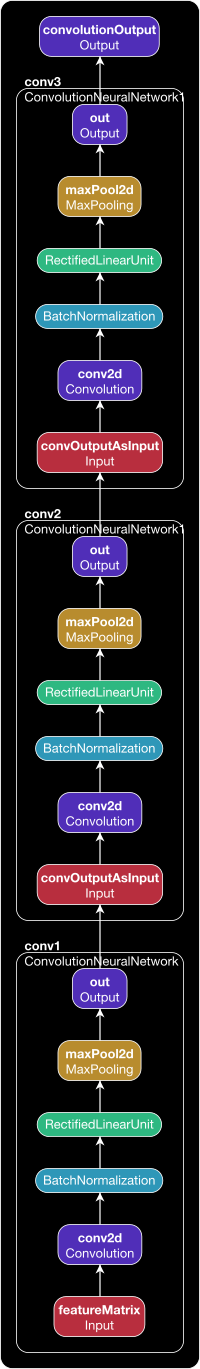
\includegraphics[width=\linewidth]{cnn.png}\caption{CNN Architecture} 
The CNN network accepts an input 2D feature vector of size 10 by 8000.
This input is passed through a convolution layer, followed by a maxpooling layer.
This is repeated two more time and at the end it outputs a vector of dimensions 30 by 2 by 500.

This vector is then flattened and passed to a fully connected dense neural network.
The output is a single value between 0 and 1, encoding non interaction and interaction respectively.

\subsection{Implementation}
Pytorch\sidecite{NEURIPS2019_9015} is used to implement the deep learning model.
The implementation is inspired by \emph{DELPHI}\sidecite{Li2020.01.31.929570}
and the works of \emph{Bock et. al}\sidecite{Bock200106}, \emph{Guo, Yi et. al}\sidecite{Guo843755}
and \emph{Miryala, Sravan et. al}\sidecite{Miryala201711}.

Anu provides a cli to make the entire life cycle of machine learning pipeline as user friendly as possible.
Almost all the operations can be performed with the cli automatically.
It can be used to fetch and preprocess data automatically.
After that tarining can be started using the cli and trained models are saved to disk after each epoch.
Finally predictions can be made using the trained models.
\end{document}